\documentclass[12pt,a4paper]{article}

\usepackage[utf8]{inputenc}
\usepackage[english]{babel}
\usepackage{alphabeta} 

\usepackage[pdftex]{graphicx}
\usepackage[top=1in, bottom=1in, left=1in, right=1in]{geometry}
\usepackage{titlesec}
\linespread{1.06}
\setlength{\parskip}{8pt plus2pt minus2pt}

\widowpenalty 10000
\clubpenalty 10000

\newcommand{\eat}[1]{}
\newcommand{\HRule}{\rule{\linewidth}{0.5mm}}

\usepackage{enumitem}
\setlist{nolistsep,noitemsep}
\usepackage[hidelinks]{hyperref}
\usepackage{cite}

\begin{document}

%===========================================================
\begin{titlepage}
\begin{center}

% Top 

\includegraphics[width=0.85\textwidth]{logo-FI-UNLPam.jpg}~\\[2cm]


% Title
\HRule \\[0.4cm]
{ \LARGE 
  \textbf{Apache Kafka y Recuperación del Consumidor}\\[0.4cm]
  \emph{Gestión de fallos de registro en arquitecturas orientadas a eventos}\\[0.3cm]
}
\HRule \\[1.5cm]



% Author
{ \large
  Martin Sposito Simón, Galan Laureano Facundo y Lopez Ailin Yara \\[0.1cm]
  % \texttt{xx@xx.xx}
}

\vfill

\textsc{\Large Informe para la asignatura Sistemas Distribuidos}\\[0.4cm]
\textsc{\large Ingeniería en Sistemas/Computación}\\[0.4cm]


% Bottom
{\large \today}
 
\end{center}
\end{titlepage}

\begin{abstract}
El presente informe tiene como objetivo el estudio de un flujo de pedidos con productor, broker y consumidor en la plataforma distribuida de transmisión Apache Kafka

\addtocontents{toc}{\protect\thispagestyle{empty}}
\end{abstract}

\newpage



%===========================================================
\tableofcontents
\addtocontents{toc}{\protect\thispagestyle{empty}}
\newpage
\setcounter{page}{1}

%===========================================================
%===========================================================
\section{Introducción}\label{sec:intro}

A diferencia de los sistemas de mensajería tradicionales, Apache Kafka adopta un paradigma de registro de confirmación distribuido es decir la información se gestiona como un historial de transacciones inmutable, ordenado y replicado entre múltiples servidores

% ¿Qué es un sistema distribuido?
% Un sistema distribuido~\cite{SD-book} es un conjunto de equipos independientes que actúan de forma transparente como un único equipo (ver Figura~\ref{fig:SD}).

% Su objetivo es descentralizar tanto el almacenamiento de la información como el procesamiento.

% \textbf{\textit{¿Qué ventajas aporta?}}
% Algunas de las ventajas que aporta un sistema distribuido son:

% \begin{enumerate}
% \item Mayor eficacia.
% \item Mayor tolerancia a fallos: al estar distribuida la información en nodos, en caso de que se caiga un nodo, dicha información va a encontrarse replicada en otros nodos.
% \end{enumerate}


% \begin{figure}[b]
%     \centering
%     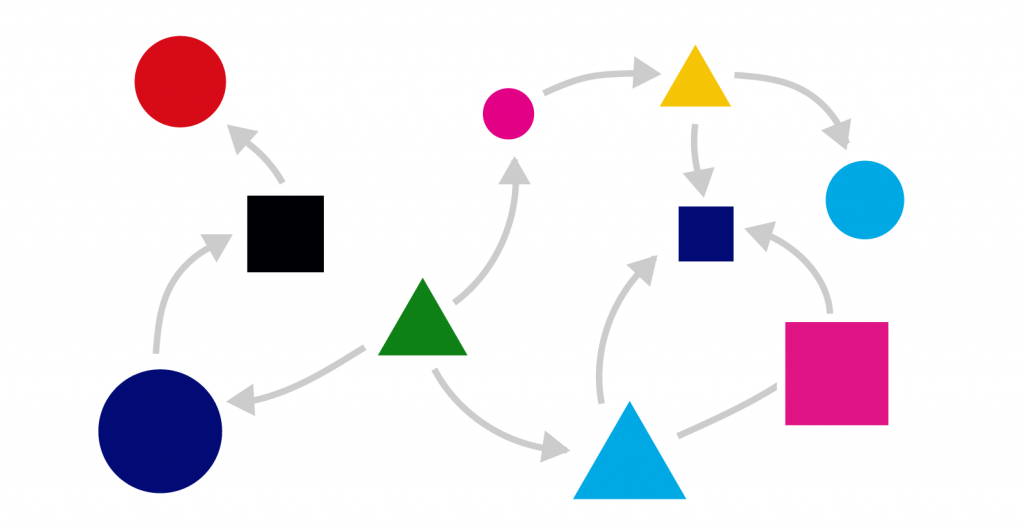
\includegraphics[width=0.75\textwidth]{SD-Imagen.png}
%     \caption{Sistema Distribuidos}
%     \label{fig:SD}
% \end{figure}

% \subsection{Apache Kafka}

% Acá va un texto.

% \subsubsection{Subsección}

% Acá va un texto.

\section{Arquitectura y Flujo de Mensajes}\label{sec:Arquitectura}

% Acá va un texto correspondiente a la sección Descripción.

\section{Mecanismos de Conf. y Garantías de Entrega}\label{sec:descrip}




\section{Análisis de Escenarios de Falla}\label{sec:Analisis}

\section{Conclusión}\label{sec:descrip}

\nocite{*} 
\bibliographystyle{ieeetr}
\bibliography{Bibliografia}


\end{document} 
